\documentclass[12pt, twoside]{article}
\usepackage[letterpaper, margin=1in, headsep=0.5in]{geometry}
\usepackage[english]{babel}
\usepackage[utf8]{inputenc}
\usepackage{amsmath}
\usepackage{amsfonts}
\usepackage{amssymb}
\usepackage{tikz}
\usetikzlibrary{quotes, angles}
\usepackage{graphicx}
%\usepackage{pgfplots}
%\pgfplotsset{width=10cm,compat=1.9}
%\usepgfplotslibrary{statistics}
%\usepackage{pgfplotstable}
%\usepackage{tkz-fct}
%\usepackage{venndiagram}
\usepackage{enumitem}
\usepackage{multicol}

\usepackage{fancyhdr}
\pagestyle{fancy}
\renewcommand{\headrulewidth}{0pt} % disable the underline of the header

\fancyhead[RO]{Name: \hspace{1.5in}}
\lhead{BECA / Dr. Huson / 10th Grade Geometry\\* 5 December 2018}

\begin{document}
\subsubsection*{Do Now: Triangle congruence proofs}
 \begin{enumerate}

 \item Given two parallel lines are intersected by a transversal,  $\overleftrightarrow{MD} || \overleftrightarrow{BC}$. $m\angle AMD =4x+5$ and $m\angle MBC=5x-7$. Find $m\angle AMD$.\\[1cm]
   \begin{tikzpicture}[scale=1.1]
     \draw [<->, thick] (-1,0)--(0,0)--(4,0);
     \draw [<->, thick] (-0.5,-0.5)--(4,4)--(4.5,4.5);
     \draw [<->, thick] (1,2)--(5, 2)--(5.5,2);
     \draw [fill] (4,4) circle [radius=0.05] node[above left]{$A$};
     \draw [fill] (5, 2) circle [radius=0.05] node[below]{$D$};
     \draw [fill] (2,2) circle [radius=0.05] node[above left]{$M$};
     \draw [fill] (0,0) circle [radius=0.05] node[above left]{$B$};
     \draw [fill] (3,0) circle [radius=0.05] node[below]{$C$};
   \end{tikzpicture} \vspace{1cm}

  \item In the diagram above, the point $M$ bisects $\overline{AB}$. If $AM=4$ find $AB$. \vspace{2cm}

 \item Given $\triangle ABC$ and $\triangle EFG$ with $\overline{AB} \cong \overline{EF}$, $\overline{BC} \cong \overline{FG}$, and $\overline{AC} \cong \overline{EG}$. \\Prove $\triangle ABC \cong \triangle EFG$ (by filling in the blanks below)\\[0.5cm]
   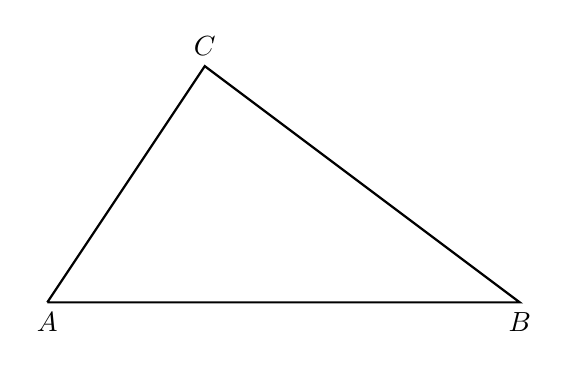
\begin{tikzpicture}
       \draw [thick]
         (2,0)node[below]{$A$}--
         (8,0)node[below]{$B$}--
         (4,3)node[above]{$C$} --(2,0);
     \end{tikzpicture}
     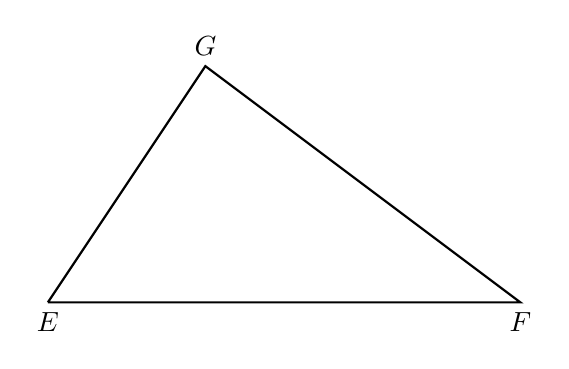
\begin{tikzpicture}%[scale=0.7]
       \draw [thick]%(0,0)node[below]{$A$}--
       (2,0)node[below]{$E$}--
       (8,0)node[below]{$F$}--
       (4,3)node[above]{$G$} --(2,0);
   \end{tikzpicture}
   \begin{multicols}{2}
     \underline{Statement} \\
     \underline{Reason}
   \end{multicols}
   \begin{multicols}{2}
     \raggedcolumns
     \begin{enumerate}[label={\arabic*)}]
       \item $\triangle ABC$, $\triangle EFG$
       \item $\overline{AB} \cong \overline{EF}$
       \item $\overline{BC} \cong \overline{FG}$, $\overline{AC} \cong \overline{EG}$
       \item $\triangle ABC \cong \triangle EFG$ \\
     \end{enumerate}
     \begin{enumerate}[label={\arabic*)}]
       \item Given
       \item \rule{4cm}{0.15mm}
       \item \rule{4cm}{0.15mm}
       \item \rule{4cm}{0.15mm}
     \end{enumerate}
   \end{multicols}

\newpage
\item Given two parallel lines intersect a transversal,  $\overleftrightarrow{MD} || \overleftrightarrow{BC}$. Given $\overline{MD} \cong \overline{BC}$ and $M$ is the midpoint of $\overline{AB}$. \\Prove $\triangle ADM \cong \triangle MCB$.
  \begin{center}
  \begin{tikzpicture}[scale=1.4]
    \draw [<->, thick] (-1,0)--(0,0)--(4,0);
    \draw [<->, thick] (-0.5,-0.5)--(4,4)--(4.5,4.5);
    \draw [<->, thick] (1,2)--(5, 2)--(5.5,2);
    \draw [-, thick] (4,4)--(5, 2);
    \draw [-, thick] (2,2)--(3,0);
    \draw [fill] (4,4) circle [radius=0.05] node[above left]{$A$};
    \draw [fill] (5, 2) circle [radius=0.05] node[below]{$D$};
    \draw [fill] (2,2) circle [radius=0.05] node[above left]{$M$};
    \draw [fill] (0,0) circle [radius=0.05] node[above left]{$B$};
    \draw [fill] (3,0) circle [radius=0.05] node[below]{$C$};
  \end{tikzpicture}
  \end{center}
  \begin{multicols}{2}
    \underline{Statement} \\
    \underline{Reason}
  \end{multicols}
  \begin{multicols}{2}
    \raggedcolumns
    \begin{enumerate}[label={\arabic*)}]
      \item $\overleftrightarrow{MD} || \overleftrightarrow{BC}$ \vspace{0.3cm}
      \item $M$ is the midpoint of $\overline{AB}$ \vspace{0.3cm}
      \item \rule{2cm}{0.15mm} $\cong \overline{BC}$ \vspace{0.3cm}
      \item $\angle AMD \cong \angle MBC$ \vspace{0.3cm}
      \item \rule{2cm}{0.15mm} $\cong \overline{AM}$ \vspace{0.3cm}
      \item $\triangle ADM \cong \triangle MCB$  \vspace{0.3cm}
    \end{enumerate}
    \begin{enumerate}[label={\arabic*)}]
      \item \rule{4cm}{0.15mm} \vspace{0.3cm}
      \item \rule{4cm}{0.15mm} \vspace{0.3cm}
      \item Given \vspace{0.3cm}
      \item \rule{4cm}{0.15mm} \vspace{0.3cm}
      \item Definition of a midpoint \vspace{0.3cm}
      \item \rule{4cm}{0.15mm} \vspace{0.3cm}
    \end{enumerate}
  \end{multicols}
  \end{enumerate}

\newpage
  \begin{enumerate}
\subsubsection*{4.6 Homework: Triangle congruence proofs}

  \item Given $\triangle ABC$ and $\triangle EFG$ with $\angle A \cong \angle E$, $\overline{AB} \cong \overline{EF}$, and $\overline{AC} \cong \overline{EG}$. Prove $\triangle ABC \cong \triangle EFG$.\\[0.5cm]
    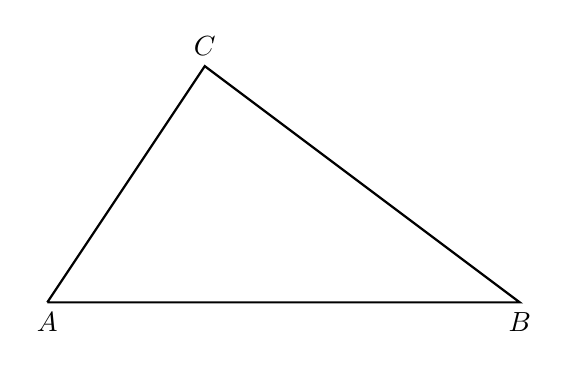
\begin{tikzpicture}
        \draw [thick]
          (2,0)node[below]{$A$}--
          (8,0)node[below]{$B$}--
          (4,3)node[above]{$C$} --(2,0);
      \end{tikzpicture}
      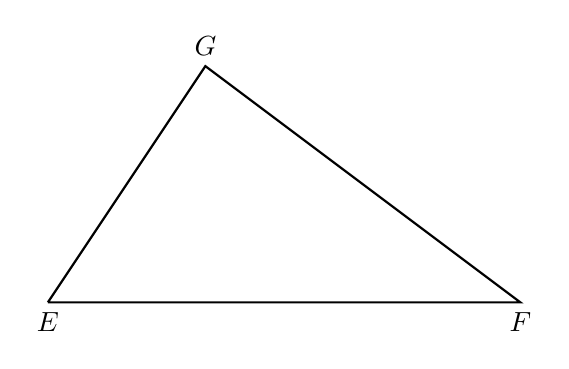
\begin{tikzpicture}%[scale=0.7]
        \draw [thick]%(0,0)node[below]{$A$}--
        (2,0)node[below]{$E$}--
        (8,0)node[below]{$F$}--
        (4,3)node[above]{$G$} --(2,0);
    \end{tikzpicture}

    \begin{multicols}{2}
      \underline{Statement} \\
      \underline{Reason}
    \end{multicols}
    \begin{multicols}{2}
      \raggedcolumns
      \begin{enumerate}[label={\arabic*)}]
        \item $\triangle ABC$, $\triangle EFG$
        \item $\angle A \cong \angle E$
        \item $\overline{AB} \cong \overline{EF}$, and $\overline{AC} \cong \overline{EG}$
        \item $\triangle ABC \cong \triangle EFG$ \\
      \end{enumerate}
      \begin{enumerate}[label={\arabic*)}]
        \item Given
        \item \rule{4cm}{0.15mm}
        \item \rule{4cm}{0.15mm}
        \item \rule{4cm}{0.15mm}
      \end{enumerate}
    \end{multicols}

  \item Given two vertical angles, $m \angle 1 = 5x+9$, $m \angle 2 = 6x-1$. Find $m \angle 1$.\\
    For full credit, check by comparing to $m\angle 2$.
      \begin{flushright}
      \begin{tikzpicture}[scale=.7]
        \draw [<->, thick] (0,-1.5)--(10,1.5);
        \draw [<->, thick] (2,3.5)--(7,-3.5);
        \node at (3,.4){1};
        \node at (6,-.6){2};
      \end{tikzpicture}
      \end{flushright}

\newpage
  \item Given $\triangle ABP$ and $\triangle JKP$ with $\angle A \cong \angle J$ and $\overline{AP} \cong \overline{JP}$. Prove $\triangle ABP \cong \triangle JKP$.\\[0.5cm]
    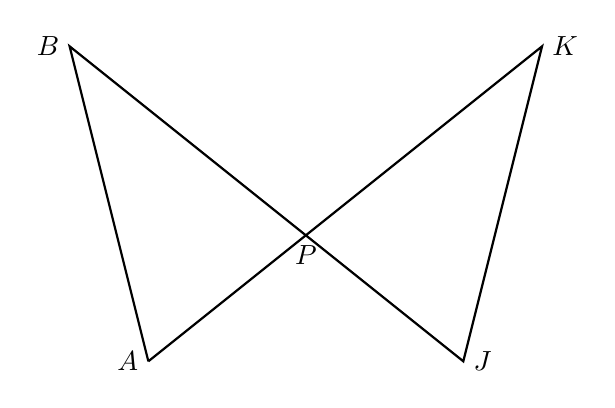
\begin{tikzpicture}
        \draw [thick]
          (-2,-1)node[left]{$A$}--
          (3,3)node[right]{$K$}--
          (2,-1)node[right]{$J$}--
          (0,0.6)node[below]{$P$}--
          (-3,3)node[left]{$B$}--(-2,-1);
      \end{tikzpicture}

    \begin{multicols}{2}
      \underline{Statement} \\
      \underline{Reason}
    \end{multicols}
    \begin{multicols}{2}
      \raggedcolumns
      \begin{enumerate}[label={\arabic*)}]
        \item $\triangle ABC$, $\triangle JKP$
        \item \rule{4cm}{0.15mm}%$\angle A \cong \angle J$ and $\overline{AP} \cong \overline{JP}$ %\vspace{0.4cm}
        \item $\angle APB \cong \angle JPK$ %

        \item $\triangle ABP \cong \triangle JKP$
      \end{enumerate}
      \begin{enumerate}[label={\arabic*)}]
        \item Given
        \item Given
        \item \rule{4cm}{0.15mm}
        \item \rule{4cm}{0.15mm}
      \end{enumerate}
    \end{multicols}

  \item Express the result to the nearest thousandth.  \vspace{1cm}

    \begin{multicols}{2}
      \begin{enumerate}
        \item $\cos 60^\circ = $ \vspace{1cm}
        \item $\tan 25^\circ =$
        \item $\sin 41^\circ = $ \vspace{1cm}
        \item $\cos 75^\circ =$

      \end{enumerate}
    \end{multicols} \vspace{1cm}

  \item Find the image of $A(3,2)$ after a translation four to the right and down two. \vspace{1cm}
  \item Apply the translation $(x,y) \rightarrow (x-5,y+1)$ to the point $B(-2,-1)$. \vspace{1cm}
  \item State the translation that would map $C(6,3)$ onto $C'(5,13)$.


\newpage
\subsubsection*{List of theorem/situations for $\triangle \cong$ proofs}
  \item Vertical angles w segment bisectors
  \item Transversal corresponding
  \item Transversal with shared side on transversal
  \item Two inscribed in circle with vertical angles
  \item Inscribed in circle triangle with external angle, showing arc measure relationship
  \item Rotate triangle


\end{enumerate}
\end{document}
